% !TEX root = ../../prj4projektdokumentation.tex

\chapter{Design af distributionslinje, belastning og trinskifter}

\section{Distributionslinje}
På baggrund af foranalysen \ref{sec:ForanalyseDisb} er længden af distributionslinjen, der ønskes simuleret, valgt til 60 km. Ud fra databladet for den valgte kabeltype ses at der  vil være 0,1 $\Omega$ /km og 0,219 mH/km, se bilag B1. For at kunne simulere disse værdier er opbygget et kredsløb med 6,2 $\Omega$ modstand i serie med en 13,6 mH spole. Dette stemmer overens med teorien for korte transmissionslinjer, hvor kun modstand og spolevirkning indgår i modellen. Modellen ses på figur \ref{fig:Kortlinjemodel} og gælder for linjer op til 80 km. 

\begin{figure}[htbp] % (alternativt [H])
	\centering
	\includegraphics[width=0.4\textwidth]{Figure/Kortlinjemodel2}
	\caption{Model for kort transmissionslinje}
	\label{fig:Kortlinjemodel}
\end{figure}


Distributionslinjen er implementeret på et printkort, hvorpå to spoler og to modstande er monteret i serie for at opnå de ønskede værdier for 'kablet'. Med en kabellængde på 60 km burde modstanden være 6 $\Omega$ og spolen 13,14 mH. På baggrund af tilgængelighed på skolens lager blev den realiserede modstand 6,2 $\Omega$ og den realiserede spole 13,6 mH. Der er desuden monteret en 1 $\Omega$ modstand i serie. Denne giver mulighed for at placere en Måleenhed til at overvåge denne del af systemet. Det færdige print til simulering af distributionslinje ses på figur \ref{fig:Disblinje}

\begin{figure}[H] 
	\centering
	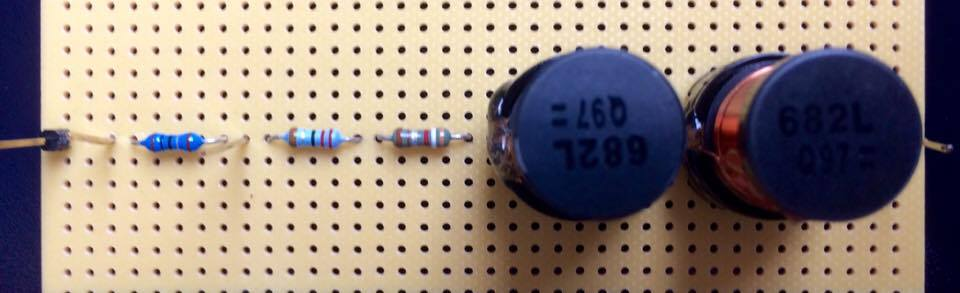
\includegraphics[width=0.7\textwidth]{Figure/Distributionslinje}
	\caption{Simulering af distributionslinje}
	\label{fig:Disblinje}
\end{figure}
